%!TEX root = ../thesis.tex

\chapter[introduction]{Introduction}\label{chp:introduction}

% ~9 pages

% Information overlead + administrative burden + lack of resources + rapid scientific progress in medicine and healthcare
In an era where technology increasingly intertwines with healthcare, artificial intelligence is on the verge of becoming part of standard medical practice. 
Growing administrative burdens, rapid scientific progress in medicine, and ageing populations have created a need to rethink how medical professionals are best enabled to successfully do their job. 
The application of artificial intelligence in medical decision-making, particularly in diagnosing and recommending treatments, is likely to hold significant potential for improving patient outcomes by reducing the effect of these issues. 
However, this prospect also raises concerns related to the reliability of such models as their decisions impact critical aspects of human health and well-being.

\todo[inline]{Can we find a better example than the Rhind Papyrus? It could be more on-point with decision-making and more well-known. Ideally, weave in an example of a failure of such technology.}
The evolution of technology to support and automate human decision-making can be traced back to the development of algorithms and mathematical techniques by many ancient civilizations. 
One example is the Egyptian Rhind Mathematical Papyrus, dated around 1550 BCE. It contains various mathematical techniques for calculations involving as multiplication, division, and fractions which were used for practical purposes like measuring land, constructing buildings, and sharing resources \cite{georges_universal_2001}. 
Concurrently, the Babylonians developed a sophisticated system of mathematics, including algorithms for solving quadratic equations, calculating areas of shapes, and numerical methods for approximating square roots \cite{fowler_square_1998}. 

However, these new tools also brought new challenges. The Babylonian system of mathematics did not formalize the difference between rational and irrational numbers often leading to approximation errors and the common practice of approximating $\pi$ with 3. Besides system limitations, human error was also a factor in the application of the new tools. The Plimpton 322 clay tablet, for instance, contains several errors presumably made by a novice in Babylonian mathematics \cite{britton_plimpton_2011} (\cref{fig:plimpton_332}).
These examples highlight the importance of understanding the limitations of technology, even in ancient times.

\begin{figure}[t]
    \centering
    
\includegraphics[width=0.80\textwidth]{plimpton_322.png}
    \caption{Technology is difficult. The author of the Plimpton 322 clay tablet ($\sim$1800 BCE) made several errors when listing Pythagorean triplets, presumably struggling to grasp Babylonian mathematics.}
    \label{fig:plimpton_332}
\end{figure}

While the quest to ease human decision-making has been ongoing for thousands of years, it was not until 1642 that the first mechanical calculator was successfully built by Blaise Pascal. And while the idea of a programmable computer with applications beyond pure arithmetic was first proposed by Ada Lovelace in 1843, 
it was not until the 1940s and 50s that % / 
% it took one-hundred years before / 
the first programmable, electronic, general-purpose digital computers were developed, starting with the ENIAC in 1945 \cite{georges_universal_2001} (\cref{fig:eniac_programmers}). 
Initially used for computing artillery trajectories, as they became more accessible general-purpose computers were adopted widely across society for various applications in the sciences, in industry and in healthcare.
The societal changes brought about by the widespread adoption of computer technology through the latter half of the 20th century have been so profound that some scholars refer to the current era as the information age \cite{georges_universal_2001, harari_sapiens_2011}.

\begin{figure}[t]
    \centering
    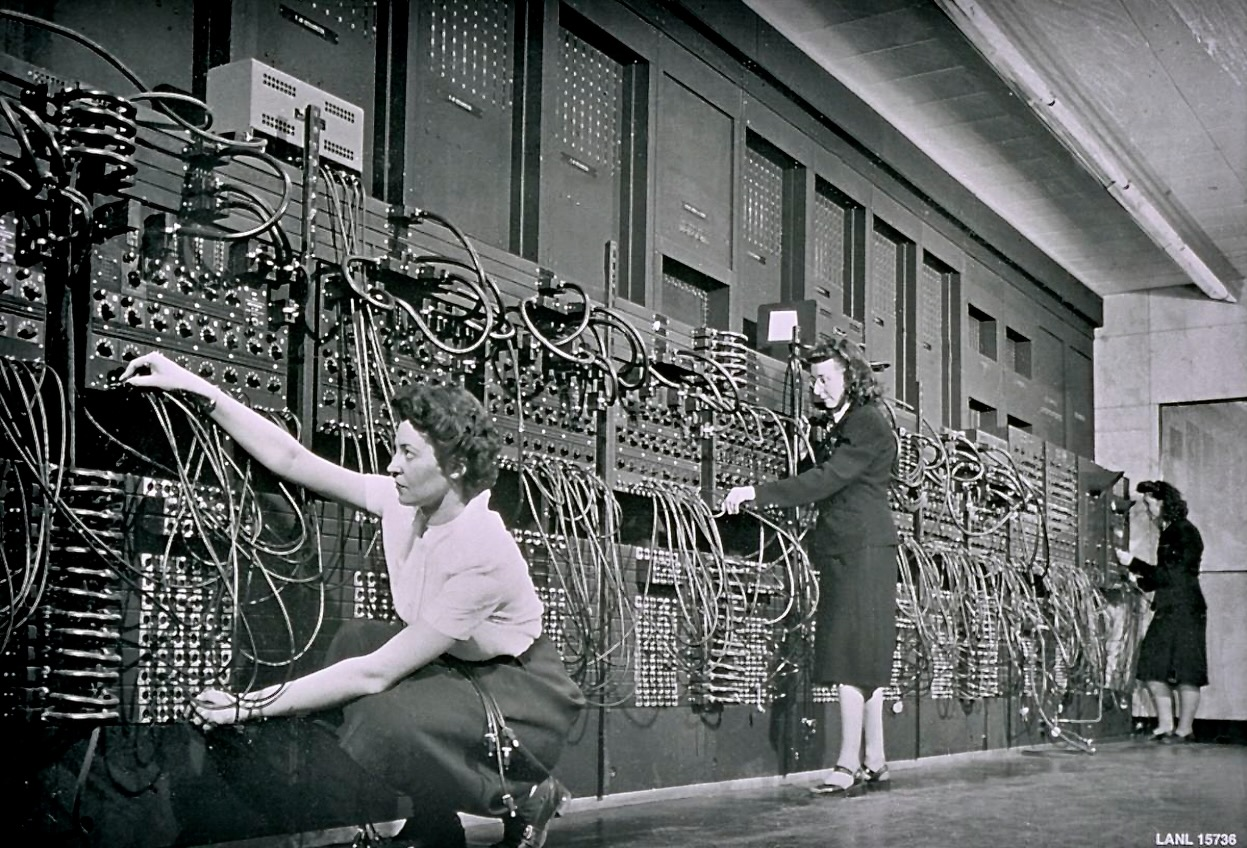
\includegraphics[width=0.95\textwidth]{eniac_programmers.jpeg}
    \caption{Ruth Lichterman (left) and Marlyn Wescoff (middle) were two of the female programmers of the ENIAC. Photo: \copyright Corbis/ Getty Images.}
    \label{fig:eniac_programmers}
\end{figure}

With the advent of the internet and the widespread adoption of digital technologies, the amount of data available to decision-makers has grown exponentially. 
This has led to a surge of interest in the scientific field of machine learning, specifically deep learning, subfields of artificial intelligence that focus on developing algorithms that can learn from data and make predictions to guide decisions based on that knowledge. 
Such methods have set new standards for the performance of computer systems in various domains, including speech recognition, computer vision, and natural language processing \cite{lecun_deep_2015}.
In recent years, machine learning has also been applied within healthcare, where it has shown promising results in tasks such as medical imaging \cite{lundervold_overview_2019}, drug discovery \cite{chen_rise_2018}, and clinical decision support \cite{cite15, cite14}.

However, these technologies come with the same risks as did previous generations, and in some cases, they may exacerbate them.
In 2018, the first incident of a self-driving car killing a pedestrian took place in Tempe, Arizona. 
The car, an SUV operated by Uber, was driving in autonomous mode when it struck a pedestrian crossing the street, pushing her bicycle. 
According to the investigation by the National Transportation Safety Board, the car's sensors detected the pedestrian $5.6$ seconds before the crash, but it did not correctly predict her path or reduce the SUV's speed (\cref{fig:uber_nhsa_accident}). 
Specifically, during those seconds, the system incorrectly classified the pedestrian more than ten times, first as a vehicle, then as an unknown object and ultimately as a bicyclist, each time changing, or resetting, the predicted path. 
About one second before the crash, the system determined that a collision was imminent, but the situation exceeded the constraints within which the autonomous driving system was allowed to operate, and the car's safety driver failed to intervene \cite{nationaltransportationsafetyboardnhsa_collision_2019}. 
This incident highlights the need for autonomous systems to be able to accurately assess their own uncertainty and act accordingly; requirements that European policymakers seek to impose on applications of machine learning via the European Artificial Inteliigence Act \cite{europeancommission_briefing_2021}.

\begin{figure}
    \centering
    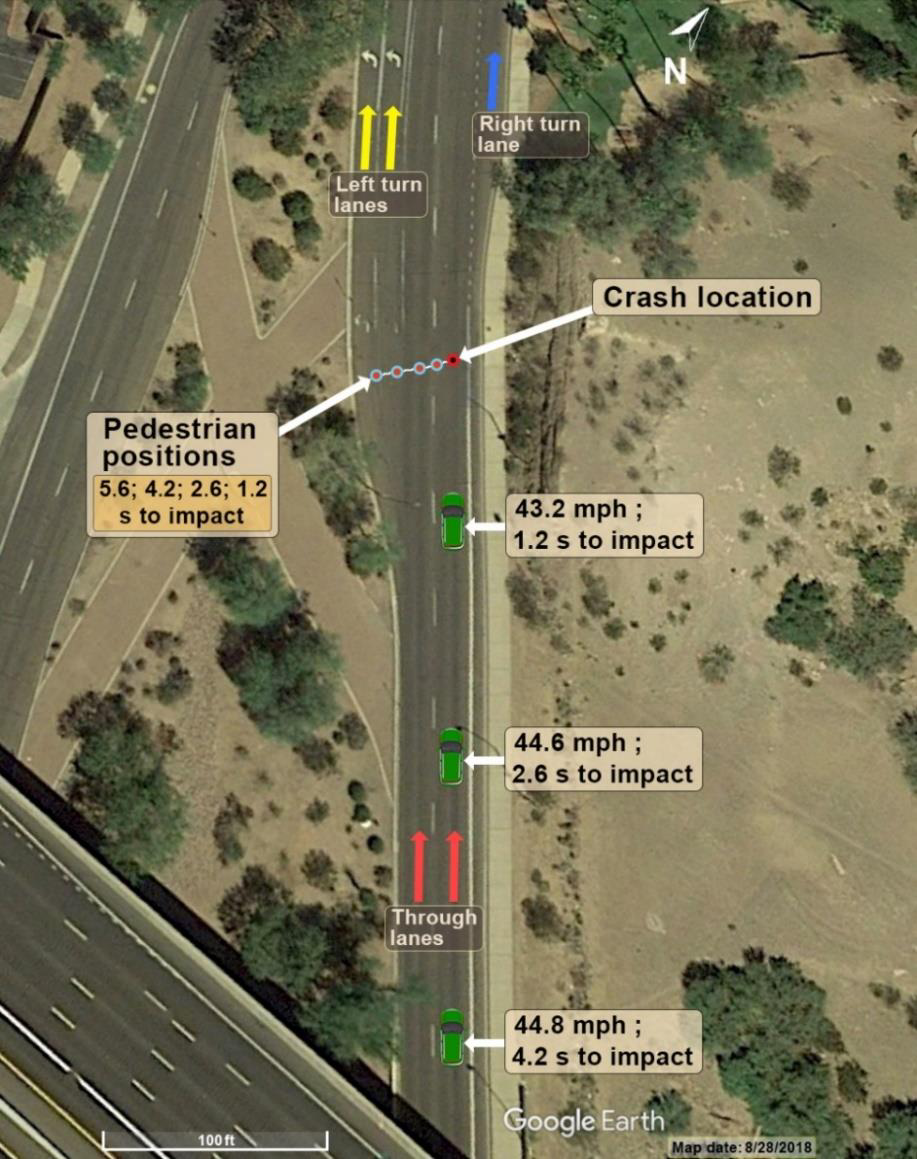
\includegraphics[width=0.95\textwidth]{uber_nhsa_accident.png}
    \caption{A pedestrian was killed by an Uber self-driving car in Tempe, Arizona in 2018. The car's sensors detected the pedestrian $5.6$ seconds before the crash, but it did not correctly predict her path or reduce the SUV's speed \cite{nationaltransportationsafetyboardnhsa_collision_2019}.}
    % \caption{Aerial view of crash location showing path of pedestrian as she attempted to cross N. Mill Avenue and movement and speed of SUV at three points before impact. Pedestrian's path shows her position from initial detection ($5.6$ seconds before impact) until impact; SUV's position is shown at corresponding times beginning $4.2$ seconds before impact \cite{nationaltransportationsafetyboardnhsa_collision_2019}.}
    \label{fig:uber_nhsa_accident}
\end{figure}

\todo[inline]{Add something here about probability theory, Bayesian modelling etc. as a warm-up for potential solutions.}



\section{Motivation: Medical conversations}

This research project was formulated and carried out in collaboration with the Danish company Corti, which develops computer software for medical decision support. 

















% The ancient Egyptians used mathematics for practical purposes like measuring land, constructing buildings, and managing resources. The Rhind Mathematical Papyrus, dated around 1550 BCE, contains various mathematical problems and techniques for calculations, such as multiplication, division, and calculations involving fractions.

% The Babylonians, around 300 BCE, developed a sophisticated system of mathematics, including algorithms for solving quadratic equations and calculating areas of shapes. The Babylonians also used numerical methods for approximating square roots.


% Greek mathematicians like Euclid (circa 300 BCE) formulated mathematical proofs and geometrical concepts that laid the foundation for algorithmic thinking. The "Euclidean algorithm," used to find the greatest common divisor of two numbers, is still taught in schools today.

% Scholars in the Islamic world made significant contributions to mathematics. Al-Khwarizmi (circa 800 CE) wrote a book called "Al-Kitab al-Mukhtasar fi Hisab al-Jabr wal-Muqabala," from which the term "algebra" is derived. The book introduced systematic methods for solving linear and quadratic equations.







\iffalse


Uncertainty is a fundamental part of human experience. The ability to understand and quantify uncertainty is crucial in making informed decisions, drawing meaningful conclusions, and assessing the reliability of predictions made from observations. Yet, capturing this ability in a mathematical model is a difficult task. 

Uncertainty estimation has long been a central topic in the field of statistics. It has traditionally been addressed through methods like confidence intervals, hypothesis testing, and Bayesian inference. Confidence intervals provide a range of plausible values for a parameter, while hypothesis testing evaluates the significance of differences between groups or variables \cite{blitzstein_introduction_2019}. Bayesian inference, on the other hand, offers a powerful framework to incorporate prior knowledge and update beliefs based on observed data using probability theory. These approaches have been extensively studied and applied in various domains, from social sciences to natural sciences, to improve the robustness and generalizability of statistical analyses \cite{gelman_bayesian_2013}. However, the widespread adoption in diverse applications of machine learning, and in particular deep neural networks, has posed new challenges in dealing with uncertainty. 

Machine learning algorithms are designed to learn patterns from data and make predictions or decisions based on those patterns. Since many applications of machine learning are concerned with real-world phenomena, it is important to understand the uncertainty associated with the predictions made by such a model. For instance, in medical diagnosis, knowing the uncertainty in a model's prediction is crucial when the consequences of a false positive or false negative can be significant. In speech recognition, knowing that a certain word was hard to transcribe for the model can help avoid misinterpretation of the transcribed text.


% The performance of machine learning models is highly dependent on the quality and quantity of data used for training. In many cases, the data used to train machine learning models are collected from the real world, and therefore, may contain biases and errors which models may learn to mirror. In addition, the complexity of modern machine learning models makes it difficult to understand how they arrive at their predictions. This is especially true for deep neural networks, which are often referred to as black-box models. The lack of interpretability makes it difficult to assess the reliability of the model's predictions.

% Modern speech processing relies on high-performance parallel computing [40, 157], large volumes of data [136, 213], and years of innovation in model design [109, 266].

% 40: High performance convolutional neural networks for document processing \cite{chellapilla_high_2006}
% 157: Imagenet classification with deep convolutional neural networks \cite{krizhevsky_imagenet_2012}
% 136: Libri-light: A benchmark for asr with limited or no supervision \cite{kahn_libri-light_2020}
% 213: Librispeech: an ASR corpus based on public domain audio books \cite{panayotov_librispeech_2015}
% 109:  Long short-term memory \cite{hochreiter_long_1997}
% 266: Attention Is All You Need \cite{vaswani_attention_2017}


\section{Machine learning and societal risk}
\todo[inline]{Discuss the role of uncertainty aware models in the context of risk.}
\cite{europeancommission_briefing_2021}


\section{Motivation: Speech recognition}


\section{Motivation: Automated medical coding}


\subsection{Uncertainty in machine learning}

\todo[inline]{Revise this section with less focus on individual methods and more focus on overall trends.}

In the context of machine learning, uncertainty is often represented by a probability distribution. The most common approach is to use Bayesian methods, where uncertainty is captured by posterior distributions over model parameters and predictions \cite{gelman_bayesian_2013}. Bayesian neural networks, for instance, offer a powerful framework to model uncertainty in deep learning architectures \cite{neal_bayesian_1995}. By incorporating prior beliefs and updating them based on observed data, these networks can produce probabilistic predictions that provide a measure of uncertainty. This is particularly useful in applications where high-confidence predictions are required, and the consequences of errors can be significant.

Recently, another interesting approach to uncertainty estimation in machine learning is the use of Monte Carlo Dropout \cite{gal_dropout_2016}. Monte Carlo Dropout leverages the idea of dropout regularization, originally employed during training to prevent overfitting. To form a prediction with associated uncertainty, Monte Carlo Dropout proposes to make multiple forward passes through the network while sampling different dropout masks for each one. This leads to obtaining a distribution of outputs for each input sample and the variance among these sampled predictions serves as a measure of uncertainty. It is computationally efficient and can be easily incorporated into existing deep learning architectures, making it an attractive choice for uncertainty estimation.

Furthermore, there has been an interest in ensemble methods for uncertainty estimation \cite{lakshminarayanan_simple_2017}. Ensembles combine the predictions of multiple models to obtain a more robust and calibrated uncertainty measure. Bagging and boosting techniques, which have been widely used in the field of statistics, have found their way into the realm of machine learning for uncertainty estimation as well. By training multiple models with different initialization or using diverse learning algorithms, ensembles can capture different sources of uncertainty, thereby providing a comprehensive assessment of the overall uncertainty in the predictions.

% We compare our framework with several major related lines of work. First, our work focuses on the quantification of epistemic uncertainty, which refers to the errors coming from the inadequacy of the model or data noises. This is different from aleatoric uncertainty, which refers to the intrinsic stochasticity of the problem [87, 91, 112, 59, 34], or predictive uncertainty which captures the sum of epistemic and aleatoric uncertainties (but not their dissection) [89, 92, 12, 3, 22]. Regarding epistemic uncertainty, a related line of study is deep ensemble that aggregates predictions from multiple independent training replications [76, 70, 38, 8, 89]. This approach, as we will make clear later, can reduce and potentially quantify procedural variability, but a naive use would require demanding retraining effort and does not address data variability. Another line is the Bayesian UQ approach on neural networks [41, 2]. This regards network weights as parameters subject to common priors such as Gaussian. Because of the computation difficulties in exact inference, an array of studies investigate efficient approximate inference approaches to estimate the posteriors [40, 46, 16, 31, 30, 90, 74, 53]. While powerful, these approaches nonetheless possess inference error that could be hard to quantify, and ultimately finding rigorous guarantees on the performance of these approximate posteriors remains open to our best knowledge.

% 87: 
% 91: 
% 112:
% 59: 
% 34: 

% 89: 
% 92: 
% 12:
% 3: 
% 22: 

% 76: 
% 70: 
% 38: 
% 8: 
% 89: X

% 41: 
% 2: 

% 40:
% 46:
% 16:
% 31:
% 30:
% 90:
% 74:
% 53:



\section{Scope of the thesis}

The complete set of research published as part of this project covers a varied set of topics. One group of the produced studies is concerned with generative latent variable models and their applications to uncertainty estimation and speech modelling \cite{havtorn_hierarchical_2021,havtorn_benchmarking_2022,bergamin_modelagnostic_2022}. Another group of studies is concerned with self-supervised speech representation learning and automatic speech recognition \cite{borgholt_scaling_2021,borgholt_we_2021,mohamed_selfsupervised_2022,borgholt_brief_2022}. A final group deals with applications within the medical domain including recognition of stroke cases in calls to medical helplines \cite{wenstrup_retrospective_2023} and medical coding of clinical notes \cite{edin_automated_2023}. 

This first part of the thesis ties together these different studies by providing a high-level overview of the research topic and summarizing the main contributions of the thesis.



\iffalse

General challenges in uncertainty estimation:
\begin{enumerate}
    \item \textbf{Accuracy}: The uncertainty estimation method should be accurate.
    \item \textbf{Interpretability}: The uncertainty estimation method should be interpretable.
    \item \textbf{Robustness}: The uncertainty estimation method should be robust to adversarial attacks.
    \item \textbf{Applicability}: The uncertainty estimation method should be applicable to a wide range of models without requiring extensive modifications.
    \item \textbf{Efficiency}: The uncertainty estimation method should be computationally efficient at training and prediction time.
    \item \textbf{Scalability}: The uncertainty estimation method should scale to large datasets.
\end{enumerate}







Uncertainty is a fundamental part of human experience. Yet, capturing it in a mathematical model is a difficult task. Historically, uncertainty estimation has been a central topic in the field of statistics. While classical statistical methods have provided valuable insights, they often assume well-defined probability distributions and may not fully capture the complexities of uncertainty in real-world scenarios. Moreover, they tend to rely heavily on parametric assumptions, which might not hold true for complex data with high-dimensional features and non-linear relationships. Therefore, in recent years, researchers have turned their attention towards more flexible and data-driven approaches to model uncertainty in various domains.

In the field of machine learning, uncertainty is often represented by a probability distribution. The most common approach is to use Bayesian methods, where uncertainty is captured by posterior distributions over model parameters and predictions. Bayesian neural networks, for instance, offer a powerful framework to model uncertainty in deep learning architectures. By incorporating prior beliefs and updating them based on observed data, these networks can produce probabilistic predictions that provide a measure of uncertainty. This is particularly useful in applications where high-confidence predictions are required, and the consequences of errors can be significant.

Recently, another promising approach to uncertainty estimation in machine learning is the use of Monte Carlo Dropout (MC Dropout). MC Dropout leverages the idea of dropout regularization, originally employed during training to prevent overfitting. During prediction, MC Dropout takes multiple forward passes through the network with dropout enabled, which leads to obtaining a distribution of outputs for each input sample. The variance among these sampled predictions serves as a measure of uncertainty. MC Dropout has shown remarkable success in various tasks such as image classification, object detection, and natural language processing. It is computationally efficient and can be easily incorporated into existing deep learning architectures, making it an attractive choice for uncertainty estimation.

Furthermore, there has been a surge of interest in ensemble methods for uncertainty estimation. Ensembles combine the predictions of multiple models to obtain a more robust and calibrated uncertainty measure. Bagging and boosting techniques, which have been widely used in the field of statistics, have found their way into the realm of machine learning for uncertainty estimation as well. By training multiple models with different initializations or using diverse learning algorithms, ensembles can capture different sources of uncertainty, thereby providing a comprehensive assessment of the overall uncertainty in the predictions.

Despite the progress made in uncertainty estimation for machine learning models, challenges still remain. One key concern is the interpretability of uncertainty measures. While probabilistic outputs are more informative than point estimates, effectively communicating uncertainty to end-users and decision-makers is not trivial. Developing visualization techniques and intuitive explanations for uncertainty is an ongoing area of research. Additionally, quantifying uncertainty in high-dimensional data or complex models with massive amounts of parameters requires careful consideration and efficient computational strategies.

In conclusion, uncertainty estimation is a crucial aspect of machine learning models, enabling them to make more informed and reliable predictions. Researchers continue to explore innovative techniques to better represent and quantify uncertainty, allowing for safer and more trustworthy deployment of machine learning systems in real-world scenarios.





Uncertainty is a fundamental part of human experience. Yet, capturing it in a mathematical model is a difficult task. Historically, uncertainty estimation has been a central topic in the field of statistics. Understanding and quantifying uncertainty is crucial in making informed decisions, drawing meaningful conclusions, and assessing the reliability of predictions and inferences derived from data.


In the field of statistics, uncertainty is traditionally addressed through methods like confidence intervals, hypothesis testing, and Bayesian inference. Confidence intervals provide a range of plausible values for a parameter, while hypothesis testing evaluates the significance of differences between groups or variables. Bayesian inference, on the other hand, offers a powerful framework to incorporate prior knowledge and update beliefs based on observed data using probability theory. These approaches have been extensively studied and applied in various domains, from social sciences to natural sciences, to improve the robustness and generalizability of statistical analyses.
However, the advent of machine learning and its widespread adoption in diverse applications has posed new challenges and opportunities in dealing with uncertainty. 

Machine learning algorithms are designed to learn patterns from data and make predictions or decisions based on that knowledge. In many cases, it is not enough to provide a single deterministic prediction; it is equally important to convey the level of uncertainty associated with the prediction. For instance, in medical diagnosis, knowing the uncertainty in a model's prediction is crucial when the consequences of a false positive or false negative can be significant. In autonomous driving systems, understanding uncertainty becomes essential to ensure the safety of passengers and pedestrians.

To address the uncertainty challenge in machine learning, researchers have developed various techniques to represent and quantify uncertainty. One of the common approaches is the use of probabilistic models, where uncertainty is captured in the form of probability distributions. Instead of providing a single point prediction, probabilistic models generate a range of possible outcomes along with their associated probabilities. Bayesian neural networks, Gaussian processes, and variational autoencoders are some examples of such models that have gained prominence in the quest for uncertainty-aware machine learning.

Another avenue for dealing with uncertainty in machine learning is through ensemble methods. Ensemble learning combines multiple models to improve predictive accuracy and can also provide uncertainty estimates. By aggregating the outputs of diverse models, ensemble methods can identify situations where predictions are consistent among the models, leading to higher confidence, and cases where the models disagree, indicating higher uncertainty.

As the intersection of statistics and machine learning grows increasingly important, the integration of these two domains has become an active area of research. The incorporation of probabilistic modeling and Bayesian approaches into machine learning methods opens up new possibilities for developing more robust, interpretable, and calibrated models. Moreover, the synergy of statistical techniques with deep learning, reinforcement learning, and other advanced machine learning paradigms has the potential to push the boundaries of uncertainty quantification and application even further.

In this thesis, we aim to explore and contribute to the field of uncertainty in statistics and machine learning. We will investigate state-of-the-art methods for uncertainty estimation, delve into their theoretical underpinnings, and evaluate their performance in various real-world scenarios. By gaining a deeper understanding of uncertainty and its implications, we aspire to pave the way for more reliable, trustworthy, and accountable AI systems in the future.

In the following chapters, we will begin by reviewing the relevant literature on uncertainty in both statistics and machine learning, providing a comprehensive overview of the current landscape. We will then present our proposed methodologies and empirical studies, illustrating how uncertainty quantification can enhance decision-making processes and mitigate risks in practical applications. Finally, we will conclude with a discussion of our findings, potential limitations, and future research directions in this exciting and rapidly evolving field.

\fi
\fi